% Requires: \usepackage{graphicx,tikz}
% Image paths are relative to this .tex file's location.
% Generated by: smixae latex figures  (experiment: gemma_2_2b_l12)

\begin{figure*}[t]
\centering
\noindent\makebox[\linewidth][c]{%
\begin{minipage}[t]{\linewidth}%
\vspace{0pt}\centering%
\begin{minipage}[c][4.0cm][c]{0.3267\linewidth}%
\centering%
\begin{tikzpicture}[baseline=(img.base)]
  \node[inner sep=0pt] (img) {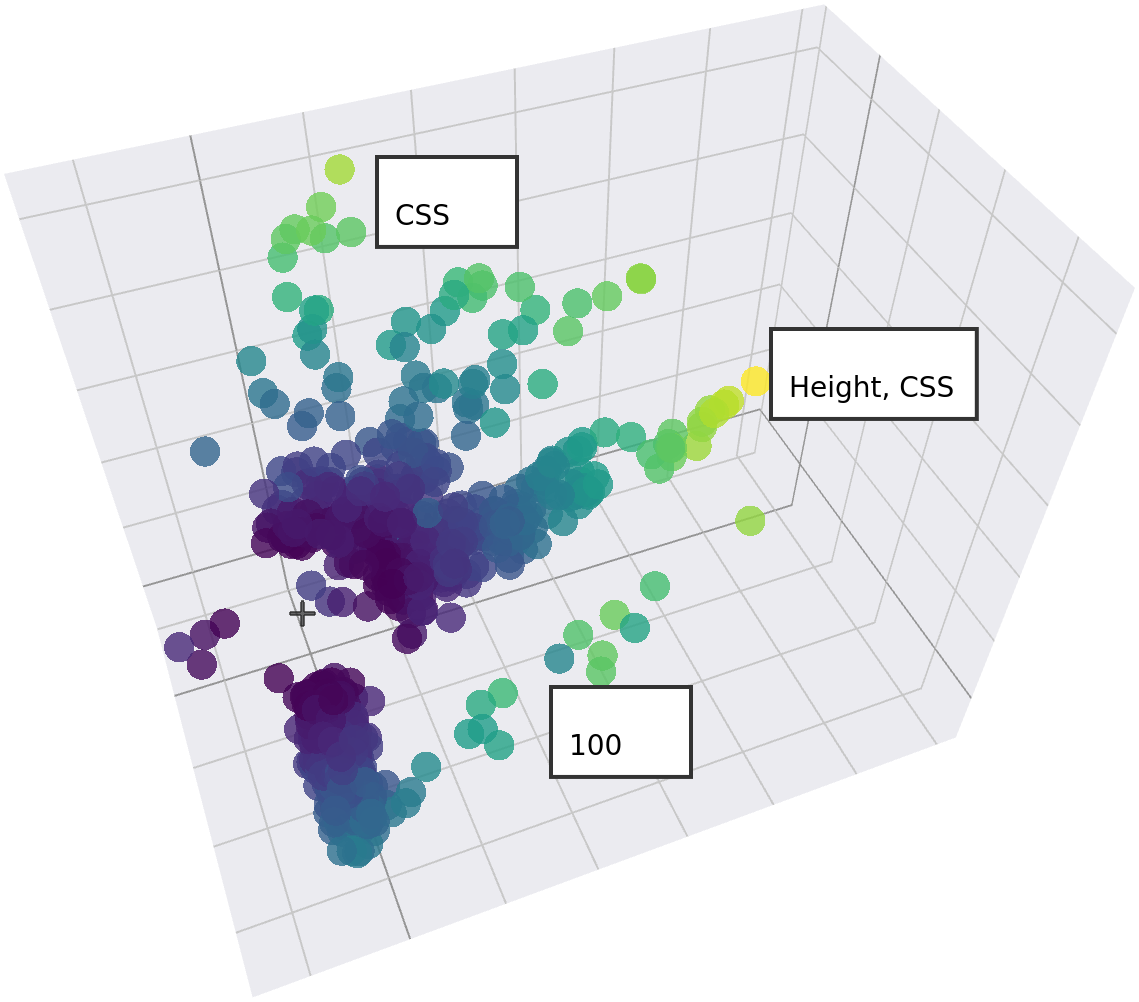
\includegraphics[width=\linewidth,height=4.0cm,keepaspectratio]{paper/camera_ready/gemma_2_2b_l12__continuity__E1359__random__cont__0.5094__scatter.png}};
  \node[anchor=north west, inner sep=2pt, overlay] at (img.north west) {\small\textbf{(a)}};
\end{tikzpicture}%
\end{minipage}%
\begin{minipage}[c][4.0cm][c]{0.3267\linewidth}%
\centering%
\begin{tikzpicture}[baseline=(img.base)]
  \node[inner sep=0pt] (img) {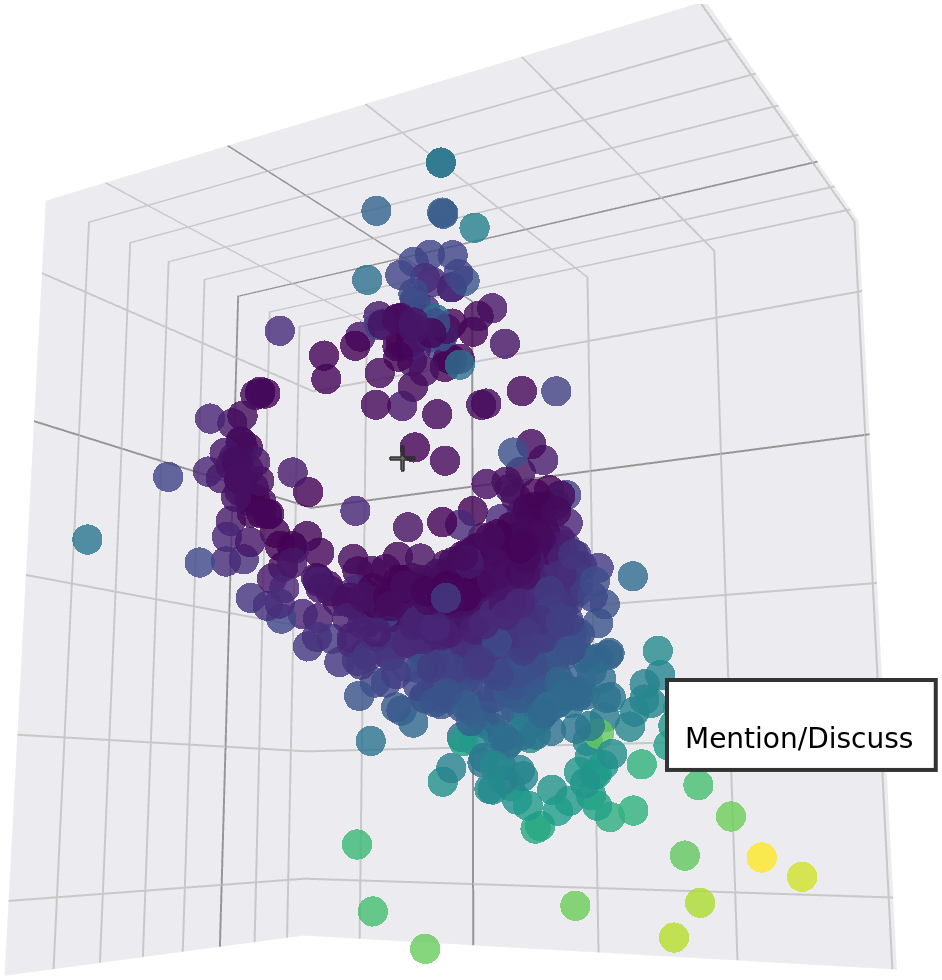
\includegraphics[width=\linewidth,height=4.0cm,keepaspectratio]{paper/camera_ready/gemma_2_2b_l12__continuity__E1568__random__cont__0.4995__scatter.png}};
  \node[anchor=north west, inner sep=2pt, overlay] at (img.north west) {\small\textbf{(b)}};
\end{tikzpicture}%
\end{minipage}%
\begin{minipage}[c][4.0cm][c]{0.3267\linewidth}%
\centering%
\begin{tikzpicture}[baseline=(img.base)]
  \node[inner sep=0pt] (img) {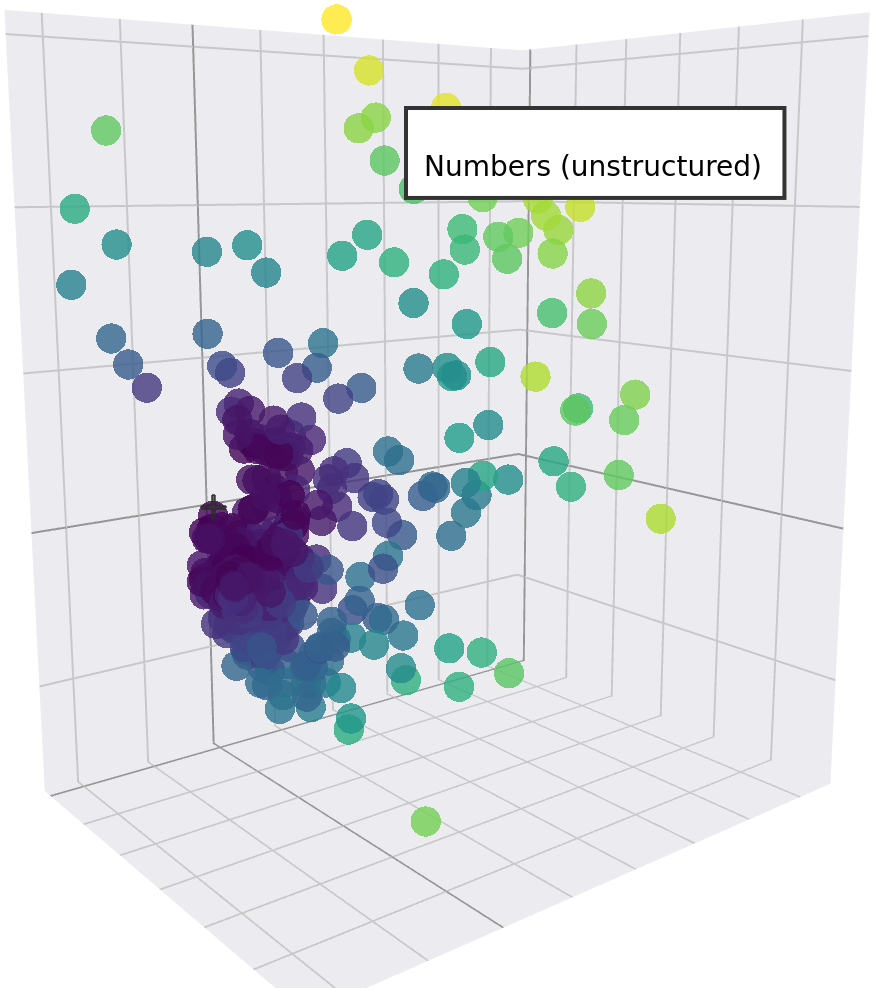
\includegraphics[width=\linewidth,height=4.0cm,keepaspectratio]{paper/camera_ready/gemma_2_2b_l12__continuity__E1578__random__cont__0.5163__scatter.png}};
  \node[anchor=north west, inner sep=2pt, overlay] at (img.north west) {\small\textbf{(c)}};
\end{tikzpicture}%
\end{minipage}%
\par\vspace{3pt}%
\begin{minipage}[c][4.0cm][c]{0.3267\linewidth}%
\centering%
\begin{tikzpicture}[baseline=(img.base)]
  \node[inner sep=0pt] (img) {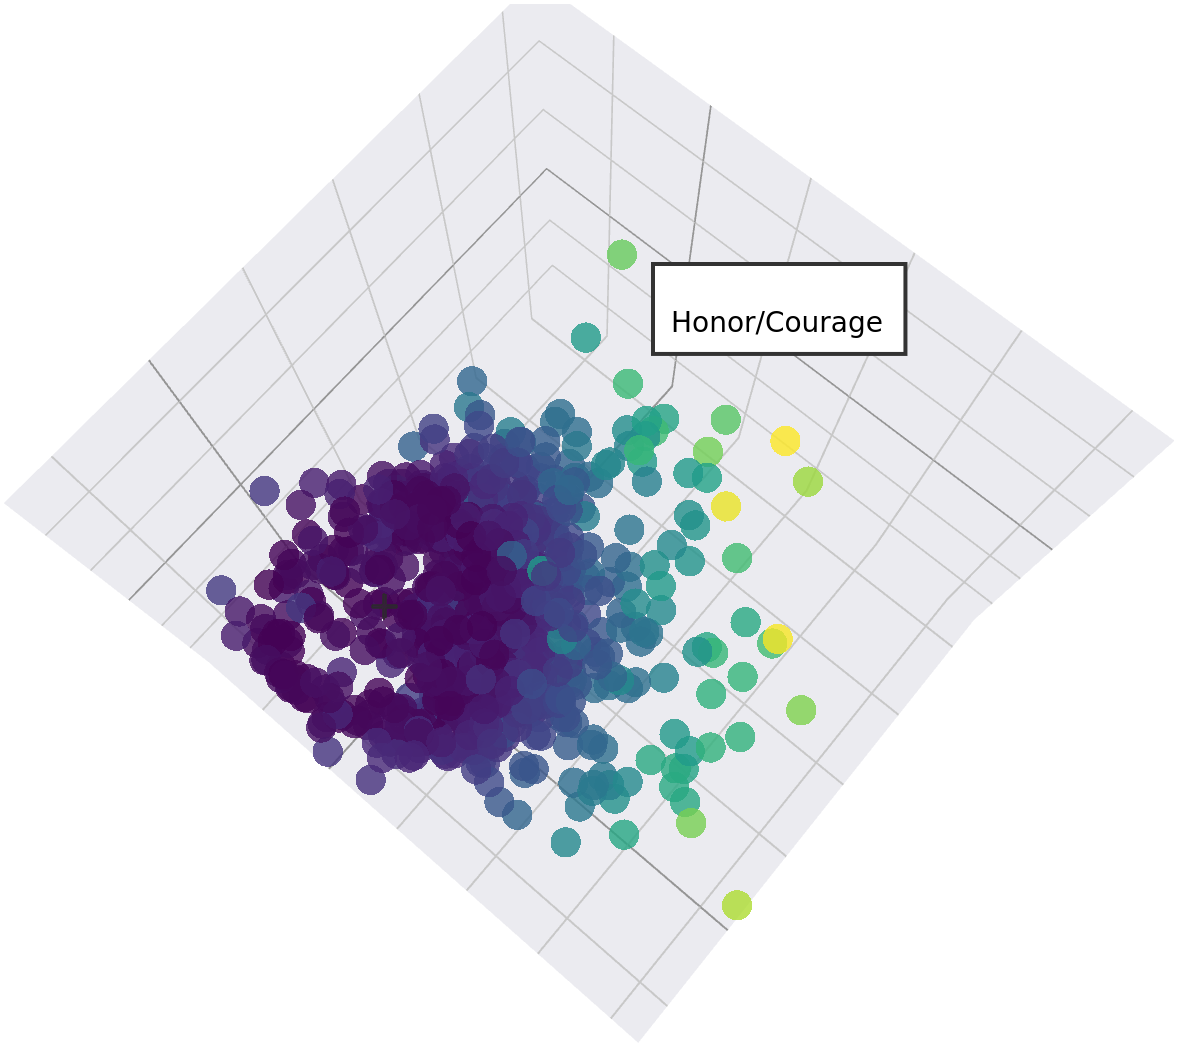
\includegraphics[width=\linewidth,height=4.0cm,keepaspectratio]{paper/camera_ready/gemma_2_2b_l12__continuity__E213__random__cont__0.4305__scatter.png}};
  \node[anchor=north west, inner sep=2pt, overlay] at (img.north west) {\small\textbf{(d)}};
\end{tikzpicture}%
\end{minipage}%
\begin{minipage}[c][4.0cm][c]{0.3267\linewidth}%
\centering%
\begin{tikzpicture}[baseline=(img.base)]
  \node[inner sep=0pt] (img) {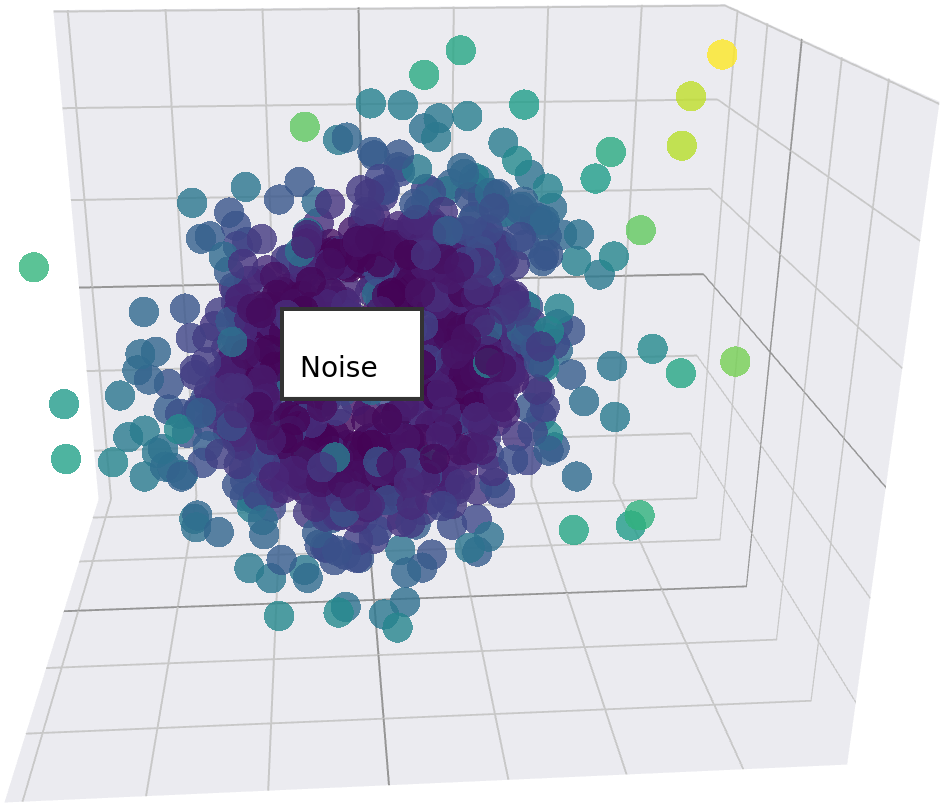
\includegraphics[width=\linewidth,height=4.0cm,keepaspectratio]{paper/camera_ready/gemma_2_2b_l12__continuity__E234__random__cont__0.3594__scatter.png}};
  \node[anchor=north west, inner sep=2pt, overlay] at (img.north west) {\small\textbf{(e)}};
\end{tikzpicture}%
\end{minipage}%
\begin{minipage}[c][4.0cm][c]{0.3267\linewidth}%
\centering%
\begin{tikzpicture}[baseline=(img.base)]
  \node[inner sep=0pt] (img) {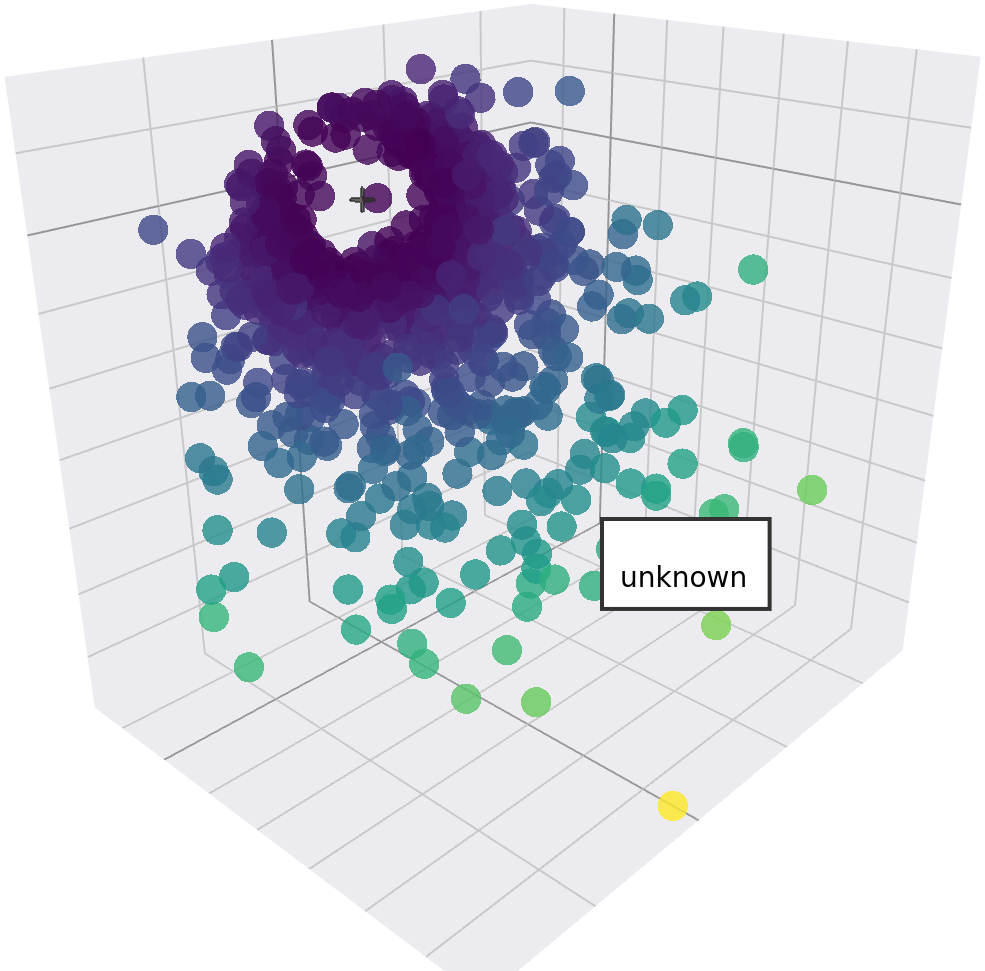
\includegraphics[width=\linewidth,height=4.0cm,keepaspectratio]{paper/camera_ready/gemma_2_2b_l12__continuity__E293__random__cont__0.3913__scatter.png}};
  \node[anchor=north west, inner sep=2pt, overlay] at (img.north west) {\small\textbf{(f)}};
\end{tikzpicture}%
\end{minipage}%
\par\vspace{3pt}%
\begin{minipage}[c][4.0cm][c]{0.3267\linewidth}%
\centering%
\begin{tikzpicture}[baseline=(img.base)]
  \node[inner sep=0pt] (img) {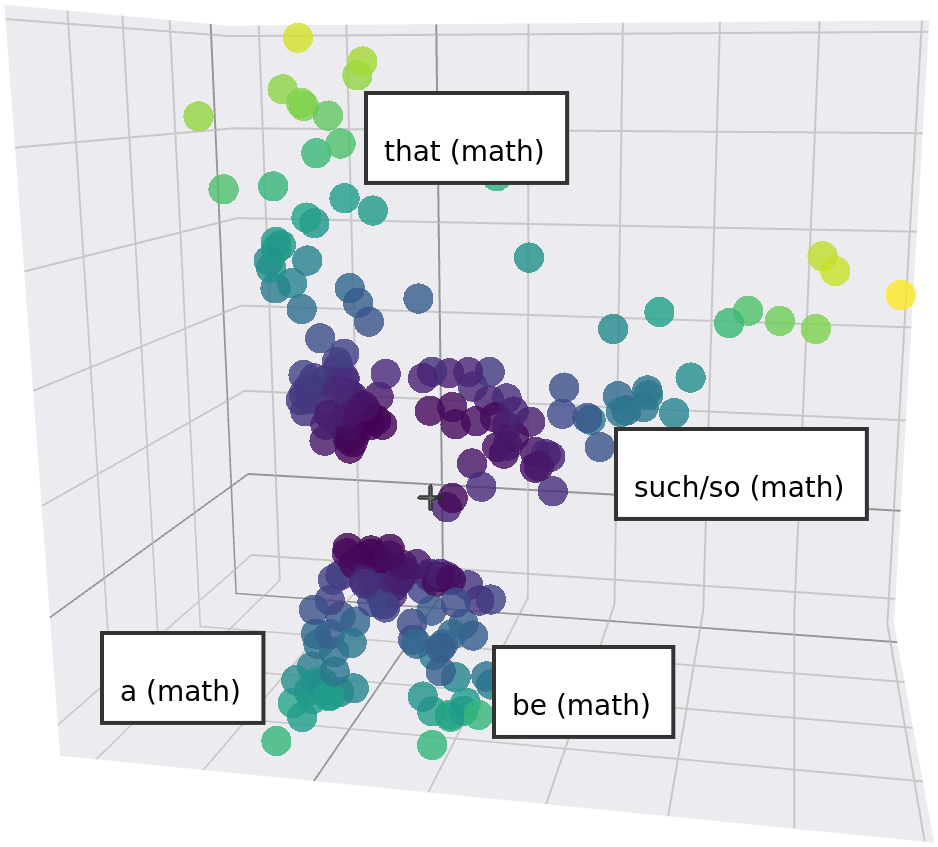
\includegraphics[width=\linewidth,height=4.0cm,keepaspectratio]{paper/camera_ready/gemma_2_2b_l12__continuity__E477__random__cont__0.6811__scatter.png}};
  \node[anchor=north west, inner sep=2pt, overlay] at (img.north west) {\small\textbf{(g)}};
\end{tikzpicture}%
\end{minipage}%
\begin{minipage}[c][4.0cm][c]{0.3267\linewidth}%
\centering%
\begin{tikzpicture}[baseline=(img.base)]
  \node[inner sep=0pt] (img) {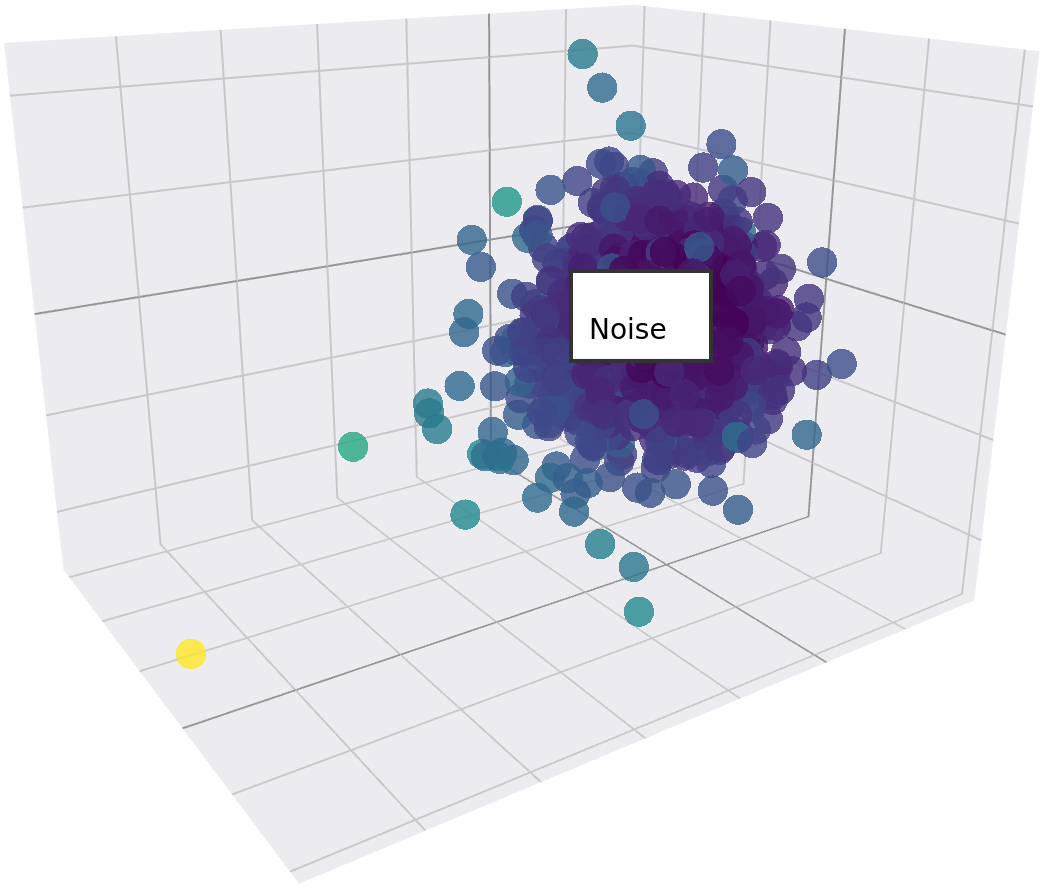
\includegraphics[width=\linewidth,height=4.0cm,keepaspectratio]{paper/camera_ready/gemma_2_2b_l12__continuity__E51__random__cont__0.3898__scatter.png}};
  \node[anchor=north west, inner sep=2pt, overlay] at (img.north west) {\small\textbf{(h)}};
\end{tikzpicture}%
\end{minipage}%
\begin{minipage}[c][4.0cm][c]{0.3267\linewidth}%
\centering%
\begin{tikzpicture}[baseline=(img.base)]
  \node[inner sep=0pt] (img) {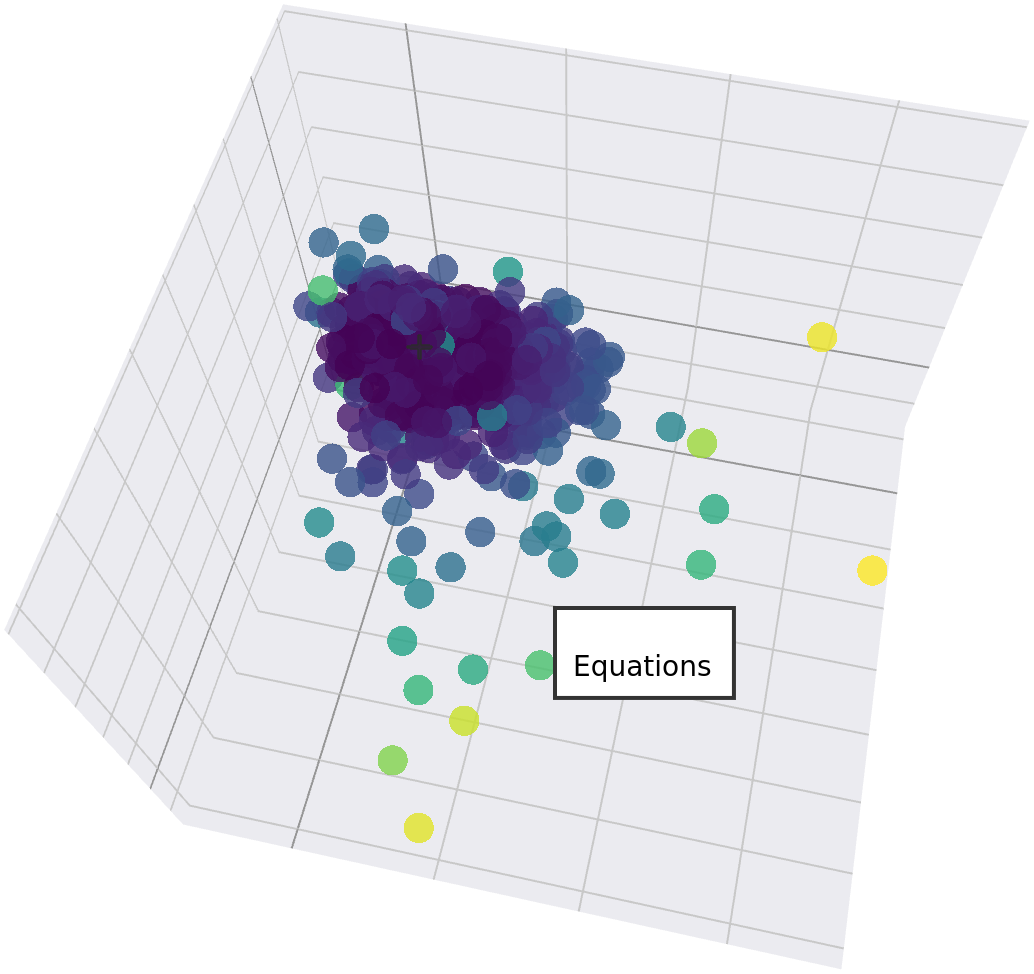
\includegraphics[width=\linewidth,height=4.0cm,keepaspectratio]{paper/camera_ready/gemma_2_2b_l12__continuity__E524__random__cont__0.4848__scatter.png}};
  \node[anchor=north west, inner sep=2pt, overlay] at (img.north west) {\small\textbf{(i)}};
\end{tikzpicture}%
\end{minipage}%
\par\vspace{3pt}%
\begin{minipage}[c][4.0cm][c]{0.3267\linewidth}%
\centering%
\begin{tikzpicture}[baseline=(img.base)]
  \node[inner sep=0pt] (img) {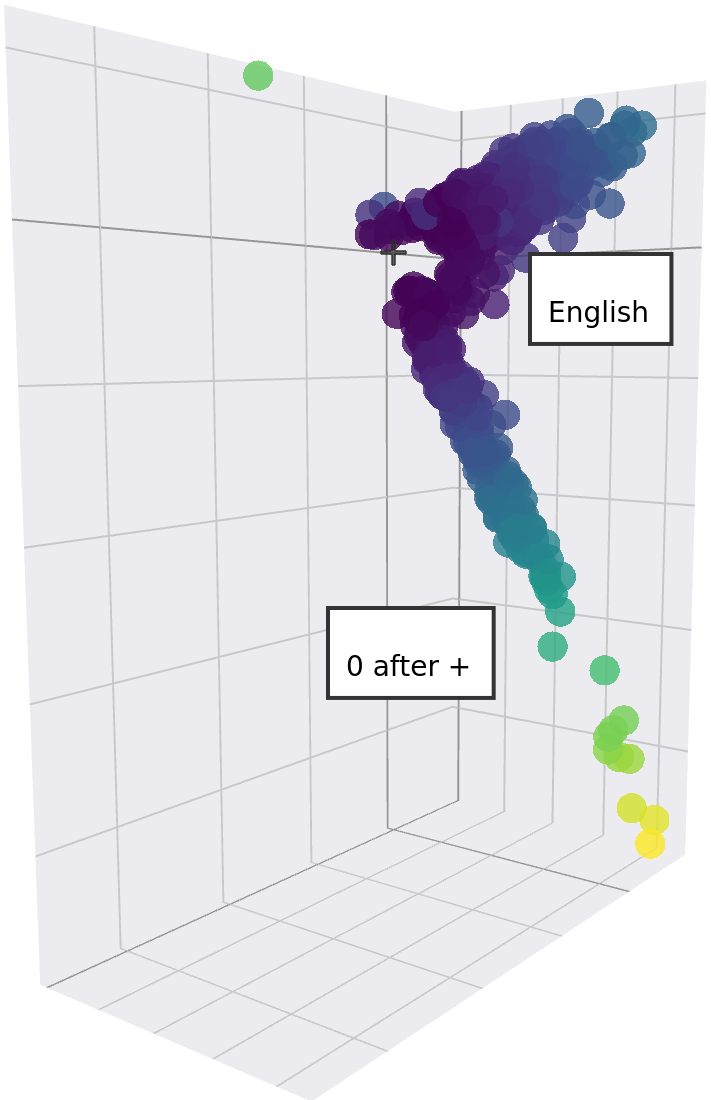
\includegraphics[width=\linewidth,height=4.0cm,keepaspectratio]{paper/camera_ready/gemma_2_2b_l12__continuity__E587__random__cont__0.4584__scatter.png}};
  \node[anchor=north west, inner sep=2pt, overlay] at (img.north west) {\small\textbf{(j)}};
\end{tikzpicture}%
\end{minipage}%
\begin{minipage}[c][4.0cm][c]{0.3267\linewidth}%
\centering%
\vspace{0pt}%
\end{minipage}%
\begin{minipage}[c][4.0cm][c]{0.3267\linewidth}%
\centering%
\vspace{0pt}%
\end{minipage}%
\par\vspace{1pt}%
{\footnotesize\textit{Random Experts (Unlabeled)}}%
\end{minipage}%
}
\caption{Gemma 2 2B, Layer 12. \textbf{Random Experts (Unlabeled)}: (a) Expert 1359, rank 1, Random Sample (Cont.\,=\,0.509). (b) Expert 1568, rank 9, Random Sample (Cont.\,=\,0.499). (c) Expert 1578, rank 4, Random Sample (Cont.\,=\,0.516). (d) Expert 213, rank 10, Random Sample (Cont.\,=\,0.430). (e) Expert 234, rank 2, Random Sample (Cont.\,=\,0.359). (f) Expert 293, rank 8, Random Sample (Cont.\,=\,0.391). (g) Expert 477, rank 7, Random Sample (Cont.\,=\,0.681). (h) Expert 51, rank 3, Random Sample (Cont.\,=\,0.390). (i) Expert 524, rank 6, Random Sample (Cont.\,=\,0.485). (j) Expert 587, rank 5, Random Sample (Cont.\,=\,0.458). Larger points denote class mean activations in the bottleneck space; smaller points are individual token activations.}
\end{figure*}
